\documentclass[14pt,fleqn]{extarticle}
\RequirePackage{prepwell-eng}

\previewoff 

\begin{document} 
\begin{snippet}
    \correct
    
    The area bounded by the curves $y^2 = 4x$ and $x^2 = 4y$ is as shown below 
    
    \begin{center}
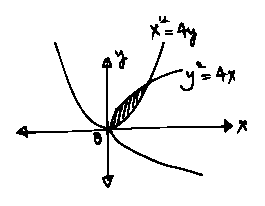
\includegraphics[scale=1.4]{figure.eps}
\end{center}
    
    
    \reason
    
    \begin{center}
  \begin{tabular}{Nc}
   \toprule
        \text{Equation} & Curve \\
   \midrule 
   x^2 = 4y & Upward opening parabola \\
    \midrule 
    y^2 = 4x & Parabola opening right \\
    \bottomrule
  \end{tabular}
\end{center}
Both parabolas touch the origin and intersect as shown. Hence, the shaded bit is the required area 
    
\end{snippet} 
\end{document} 